\documentclass{beamer}

\mode<presentation>
{
  \usetheme{default}      % or try Darmstadt, Madrid, Warsaw, ...
  \usecolortheme{default} % or try albatross, beaver, crane, ...
  \usefonttheme{serif}  % or try serif, structurebold, ...
  \setbeamertemplate{navigation symbols}{}
  \setbeamertemplate{caption}[numbered]
}

\newcommand{\Prob}{\text{Prob}}

\begin{document}
\begin{frame}{Bag of Words Model}
    \begin{columns}[T]
        \begin{column}{0.5\textwidth}
            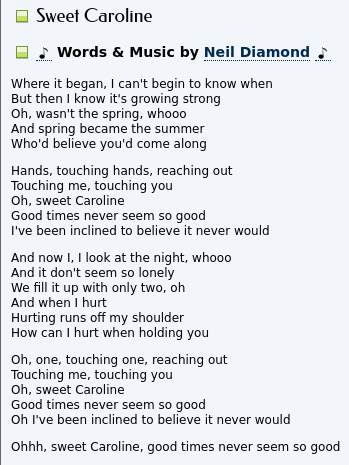
\includegraphics[width=0.9\textwidth]{sweet_caroline_lyrics.png}
        \end{column}
        \begin{column}{0.5\textwidth}
    Counts the number of times a word appears in a document and does not care about the order.
        \end{column}
    \end{columns}
\end{frame}


%%%%FRAME
\begin{frame}{Common Terminology}
    \begin{exampleblock}{Vocabulary}
        All the words we are using.
    \end{exampleblock}
        \begin{itemize}
            \item \textbf{Common Crawl (uncased)} 42B tokens, 1.9M vocab.
            \item \textbf{Common Crawl (cased)} 840B tokens, 2.2M vocab.
            \item \textbf{Twitter} 2B tweets, 27B tokens, 1.2M vocab
            \item \textbf{Wikipedia 2014 + Gigaword 5} 6B tokens 400K vocab
            \item \textbf{arXiv.org} 1,000,295 vocab.arxmliv.txt
        \end{itemize}

        \begin{exampleblock}{Labels or Classes}
            In the example these were: \textbf{Definitions, Examples, Propositions, etc}.
        \end{exampleblock}
\end{frame}

\begin{frame}
Nobody in this seminar has that (and I'm happy) but the hard part is the Data Mining.
Machine learning is fun, it's high level, rewarding and very little coding unless you want to do things from scratch.
\end{frame}

\begin{frame}
    Human language can be ambiguous
    \begin{itemize}
            \item The Pope's baby steps on gays.
            \item Scientist study whales from space.
    \end{itemize}
\end{frame}

\begin{frame}{Similarity based representations}
    ``You shall know a word by the company it keeps''\\[5mm]
    \hspace*\fill{\small John R. Firth}

\end{frame}

\begin{frame}
    \title{Distributional Similarity based representations}
    If $w_t$ is the word we care about then:
    $$Jexp(\theta) = \prod_{t=1}^T \prod_{\substack{|j|\leq m\\ j\neq 0}} \Prob(w_{t+j}| w_t; \theta)$$
    $$J(\theta) = \frac 1T \sum_{t=1}^T \sum_{\substack{|j|\leq m\\ j\neq 0}}\log \Prob(w_{t+j}| w_t; \theta)$$
\end{frame}

%%%%FRAME
\begin{frame}{How we  choose the word}
     $$p(o|c) = \frac{\exp(u_0^T v_c)}{\sum_{w=1}^V \exp(u_w^Tv_c}$$
\end{frame}


%%%%FRAME
\begin{frame}{GloVe Project}
    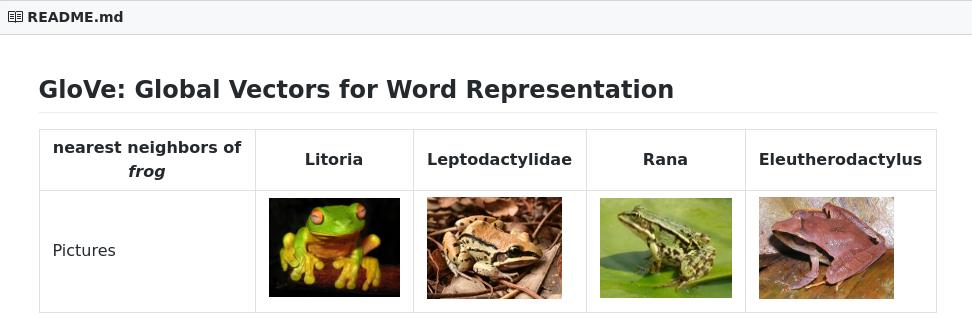
\includegraphics[width=\textwidth]{Glove_github_small.png}

\begin{figure}
   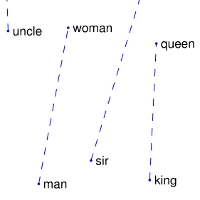
\includegraphics[width=0.29\textwidth]{man_woman_small.jpg}
   \hfill
   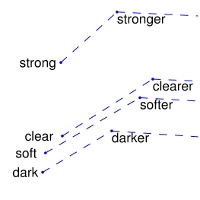
\includegraphics[width=0.29\textwidth]{comparative_superlative_small.jpg}
   \hfill
   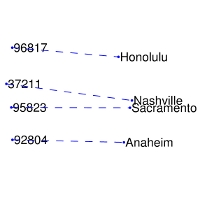
\includegraphics[width=0.29\textwidth]{city_zip_small.jpg}
\end{figure}

\end{frame}


\end{document}
